% 正态分布概率密度函数,\mu参数的变化情况
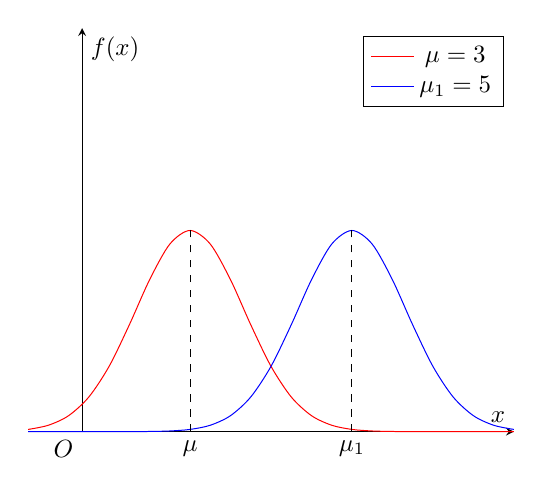
\begin{tikzpicture}[scale = 0.9]
  \begin{axis}[clip=false,xmin=-1, xmax=8,ymin=0,ymax=0.8, axis lines = middle,
    smooth, xlabel={$x$}, ylabel={$f(x)$},ticks=none]
    % mu = 2, sigma = 1
    \addplot[draw=red,domain=-1:8] {0.3989 * e^(-((x-2)^2)/2)};
    % mu = 5, sigma = 1
    \addplot[draw=blue,domain=-1:8] {0.3989 * e^(-((x-5)^2)/2)};

    % x = 2,中心
    \draw[dashed] (2,0) -- (2,0.3989);
    \node[below] at (2,0) {$\mu$};
    % x = 5,中心
    \draw[dashed] (5,0) -- (5,0.3989);
    \node[below] at (5,0) {$\mu_1$};

    % 原点标签
    \node[below left] at (0,0) {$O$};

    % 图示
    \addlegendentry{$\mu=3$}
    \addlegendentry{$\mu_1=5$}
  \end{axis}
\end{tikzpicture}
